%=================================================================

\section{Introduction}\label{sec-intro}

Shuxia is a bad girl
\gangli{is it true? Yes, very very bad!}

\subsection{Problem Statement}

1.1 Problem Summary\\
\hspace*{0.4cm}There are three types of ghastly creatures, which are called ghoul, ghost and goblins, just like the picture shows. The problem is to identify 371 data of ghastly creatures. \\
\begin{figure}[htbp]\centering
	%\graphicspath{{figures/}{mine/}}
	
\includegraphics[scale=0.3]{1.eps}
	\caption{name}
\end{figure}


1.2 Data List\\

\gangli{use description}

\begin{description}
	\item[abc] adfadaf
	\item[abc] adfadaf
\end{description}

\hspace*{0.4cm}id - id of the creature\\
\hspace*{0.4cm}bone_length - average length of bone in the creature, normalized between 0 and 1\\
\hspace*{0.4cm}rotting_flesh - percentage of rotting flesh in the creature\\
\hspace*{0.4cm}hair_length - average hair length, normalized between 0 and 1\\
\hspace*{0.4cm}has_soul - percentage of soul in the creature\\
\hspace*{0.4cm}Color - dominant color of the creature: 'white','black','clear','blue','green','blood'\\
\hspace*{0.4cm}type - target variable: 'Ghost', 'Goblin', and 'Ghoul'\\
\hspace*{0.4cm}1.3 Train Data and Test Data\\
\hspace*{0.4cm}Because this game is over, it can't submit the predictive values for testing. So divide the train data into train data and test data, and the ratio between the two is 4:1.\\

\section{Data exploration} \label{sec-data_exploration}

2.1 Data Information\\
\hspace*{0.4cm}There are 4 numerical variables and 1 categorical. And no missing values, which is nice! Numerical columns are either normalized or show a percentage, so no need to scale them. The following table is the statistical result of the attribute values.
It seems that all numerical features may be useful.\\
\begin{table}[h]  \centering
	\caption{Data Information}
	\label{tbl:data information}
	\begin{tabular}{ccccccc}
		\hline
		% after \\: \hline or \cline{col1-col2} \cline{col3-col4} ...
		& bone_length & rotting_flesh & hair_length & has_soul & color & type\\
		\hline
		count & 371.0 & 371.0 & 371.0 & 371.0 & 371 & 371 \\
		unique & NaN & NaN & NaN & NaN & 6 & 3 \\
		top & NaN & NaN & NaN & NaN & white & Ghoul \\
		freq & NaN & NaN & NaN & NaN & 137 & 129\\
		mean & 0.434160 & 0.506848 & 0.529114 & 0.471392 & NaN & NaN \\
		std & 0.132833 & 0.146358 & 0.169902 & 0.176129 & NaN & NaN \\
		min & 0.061032 & 0.095687 & 0.134600 & 0.009402 & NaN & NaN \\
		25\% & 0.340006 & 0.414812 & 0.407428 & 0.348002 & NaN & NaN \\
		50\% & 0.43891 & 0.501552 & 0.538642 & 0.466372 & NaN & NaN\\
		75\% & 0.517223 & 0.603977 & 0.647244 & 0.600610 & NaN & NaN\\
		max &  0.817001 & 0.932466 & 1.000000 & 0.935721 & NaN & NaN\\
		\hline 
		%\bottomrule
	\end{tabular}
\end{table}


\hspace*{0.1cm}2.2 Data Visualization\\
\hspace*{0.4cm}In order to observate the data intuitively, use EDA to plot the distribution of the data to find the relation between the attribute values. The followings are codes, analysis and figuers about data visualization.\\
\hspace*{0.4cm}A. Histogram\\
\hspace*{0.4cm}The figures below are the mean of the four attribute values  and the number of different color about the three types of ghastly creatures.It seems that all numerical features may be useful, but many colors are evenly distributes among the monsters. So they maybe nor very useful for analysis.\\
\begin{figure}[htbp]\centering
	%\graphicspath{{figures/}{mine/}}
	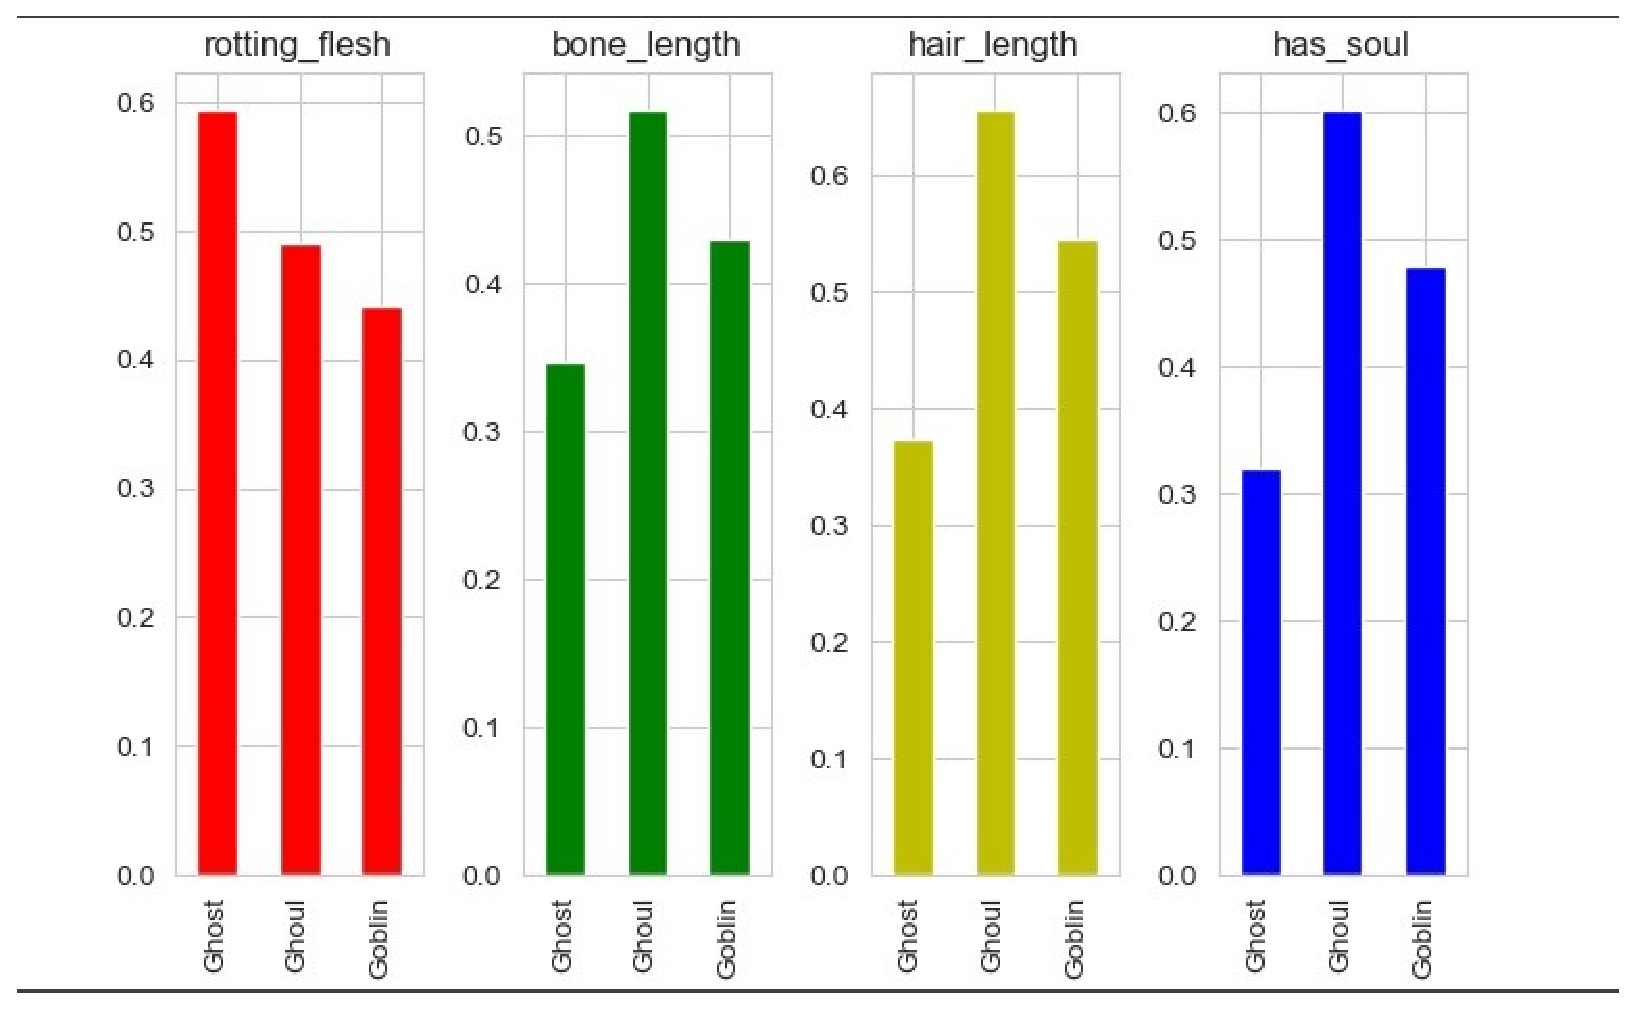
\includegraphics[scale=0.3]{2.eps}
	\caption{mean}
\end{figure}
\begin{figure}[htbp]\centering
	%\graphicspath{{figures/}{mine/}}
	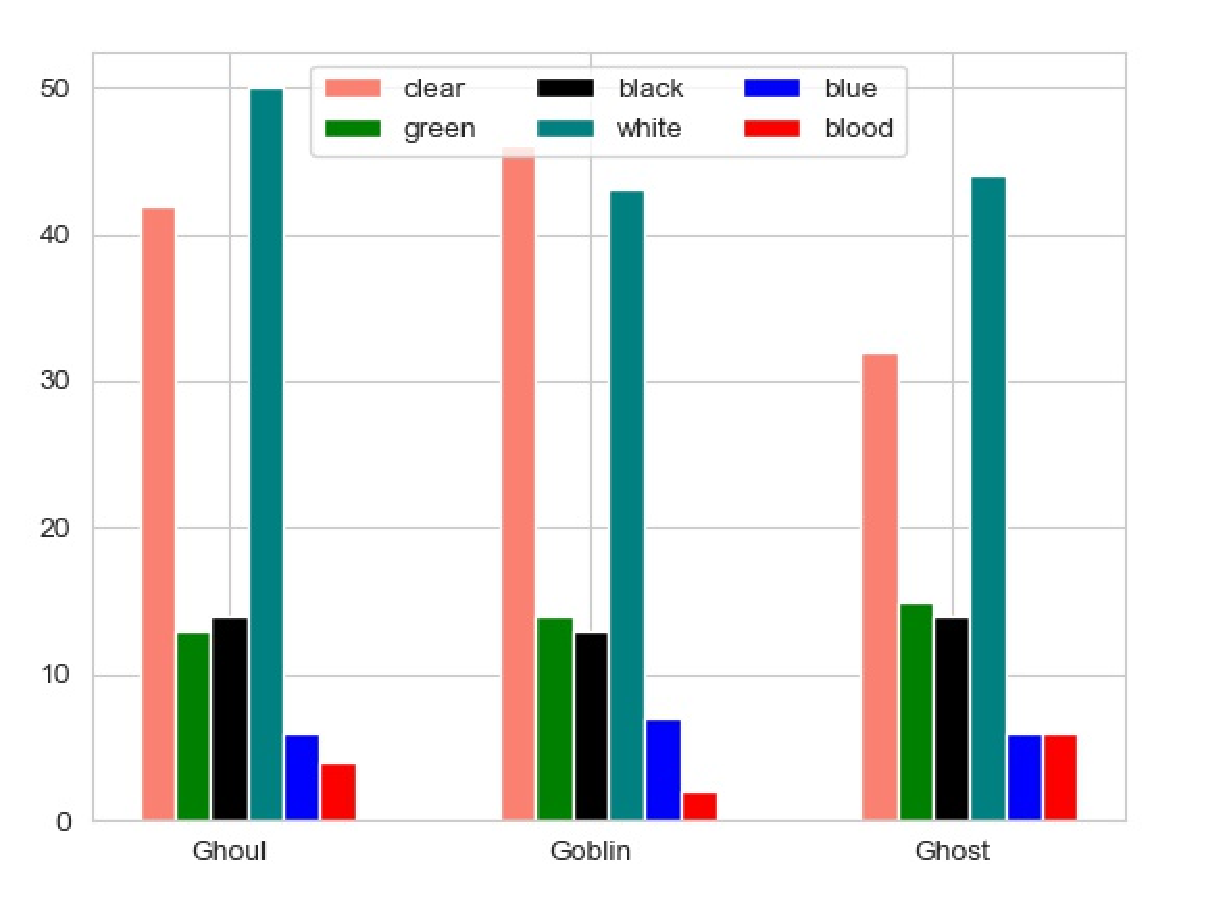
\includegraphics[scale=0.3]{3.eps}
	\caption{color}
\end{figure}


\hspace*{0.4cm}B. Boxplot\\
\hspace*{0.4cm}Through the boxplot, when analyzing the data, the boxplot can effectively help us identify the characteristics of the data: visually identify outliers in the dataset. Determine the data dispersion and bias of the data set. Through the figure, know that the two types of Ghost and Ghoul in the monster have higher discrimination on the four variables, while Goblin is in the middle position, which intersects with the other two types of features.\\
\begin{figure}[h]\centering
	%\graphicspath{{figures/}{mine/}}
	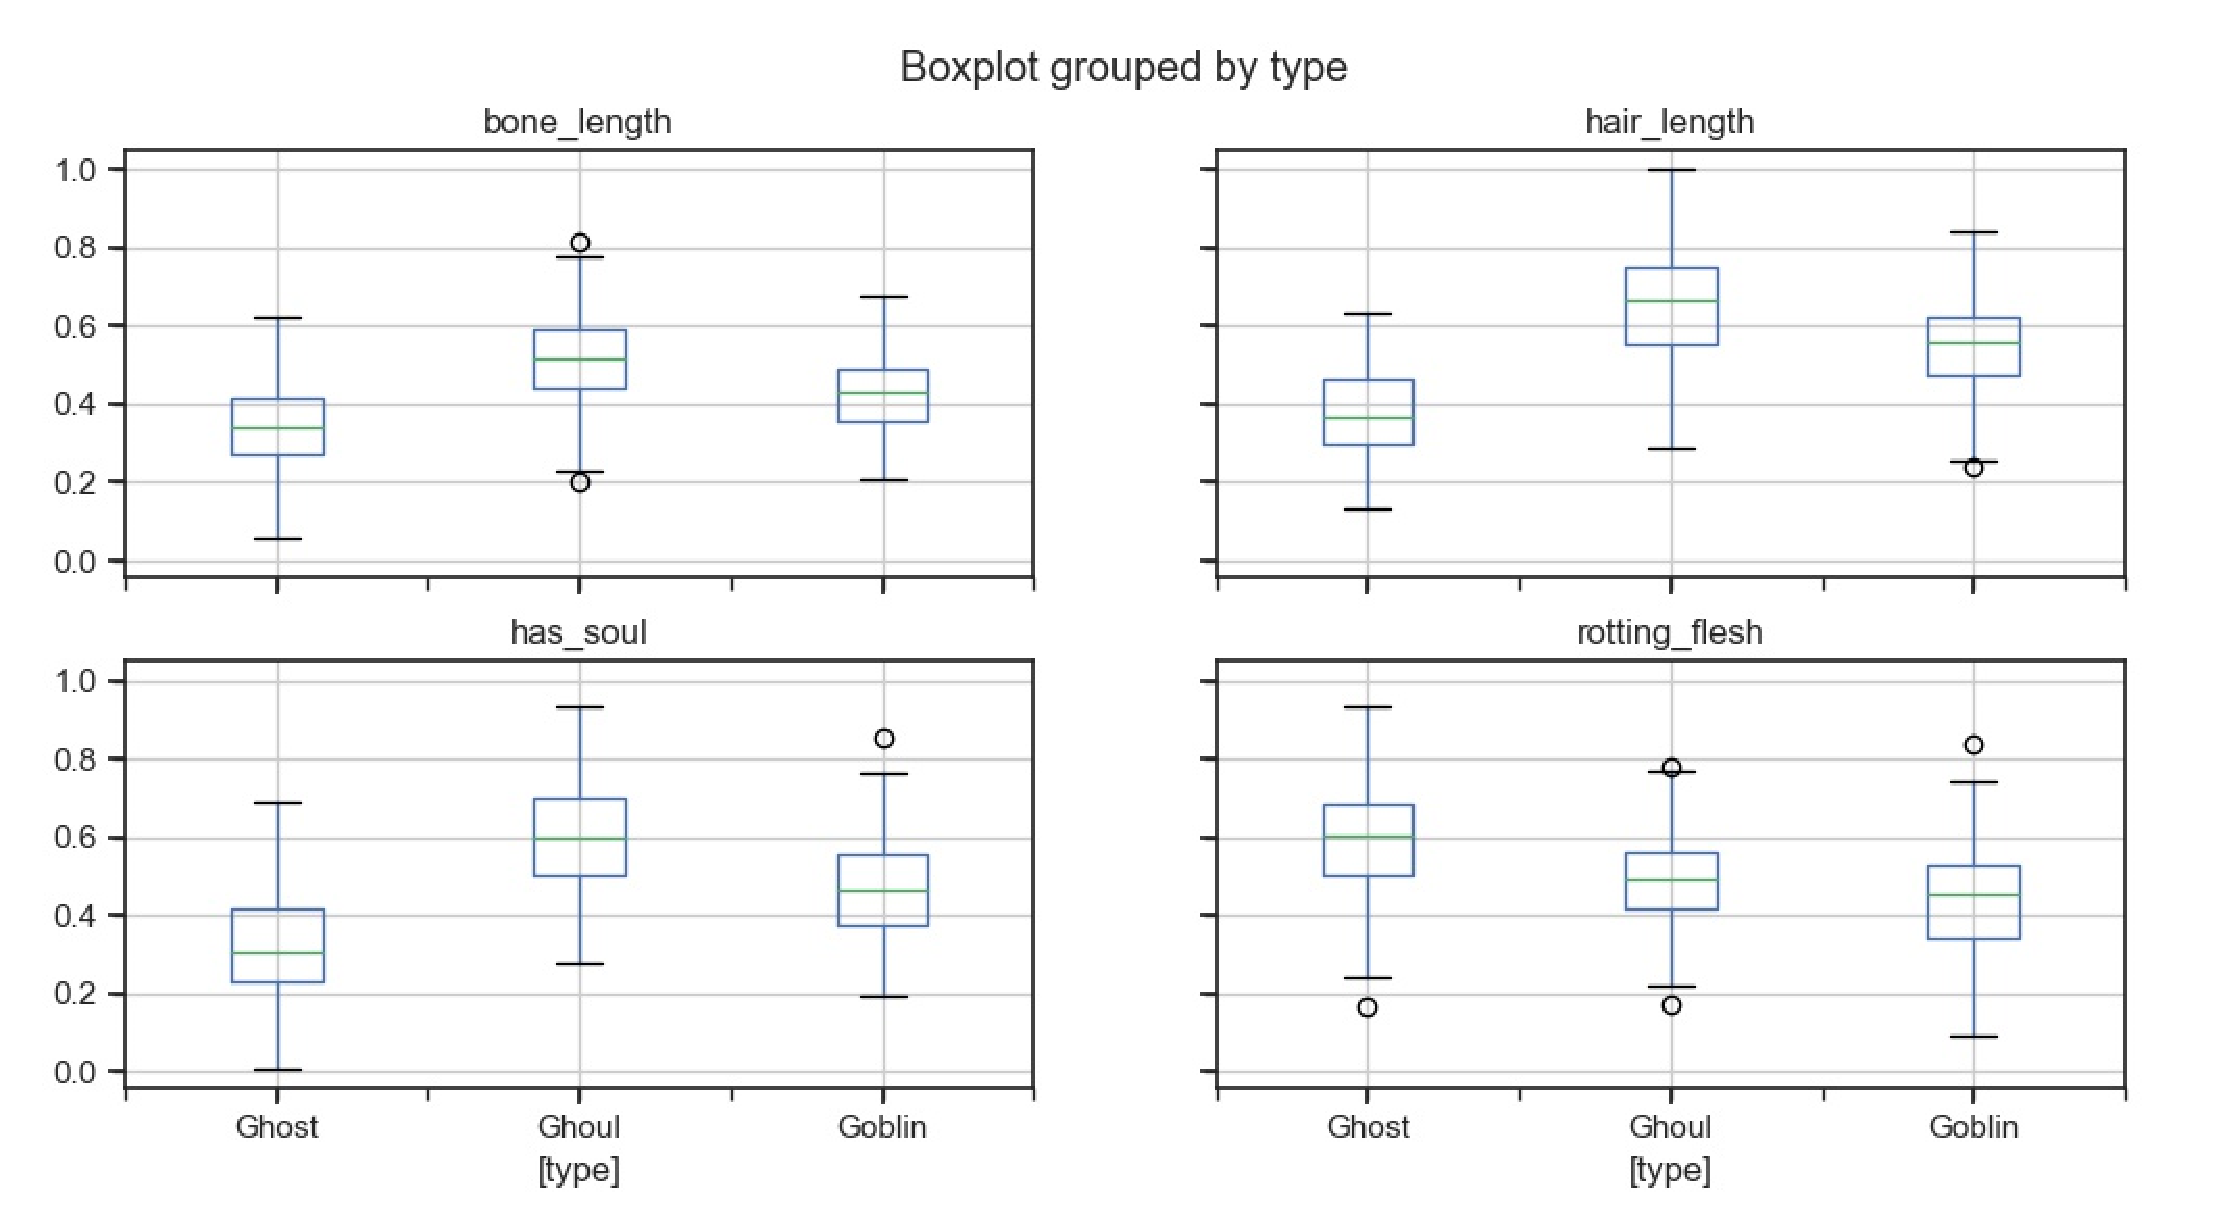
\includegraphics[scale=0.3]{4.eps}
	\caption{Boxplot Grouped by Type}
\end{figure}


\hspace*{0.4cm}C. Pairwise Plot\\
\hspace*{0.4cm}Pairwise plot is a favorite in exploratory analysis to understand the relationship between all possible pairs of numeric variables. This pairplot shows that data is distributed normally. And while most pairs are widely scattered (in relationship to the type), some of them show clusters: hair_length and has_soul, hair_length and bone_length. So it's needed to reassemble the data.\\%I decided to create new variables with multiplication of these columns and it worked great!
\begin{figure}[h]\centering
	%\graphicspath{{figures/}{mine/}}
	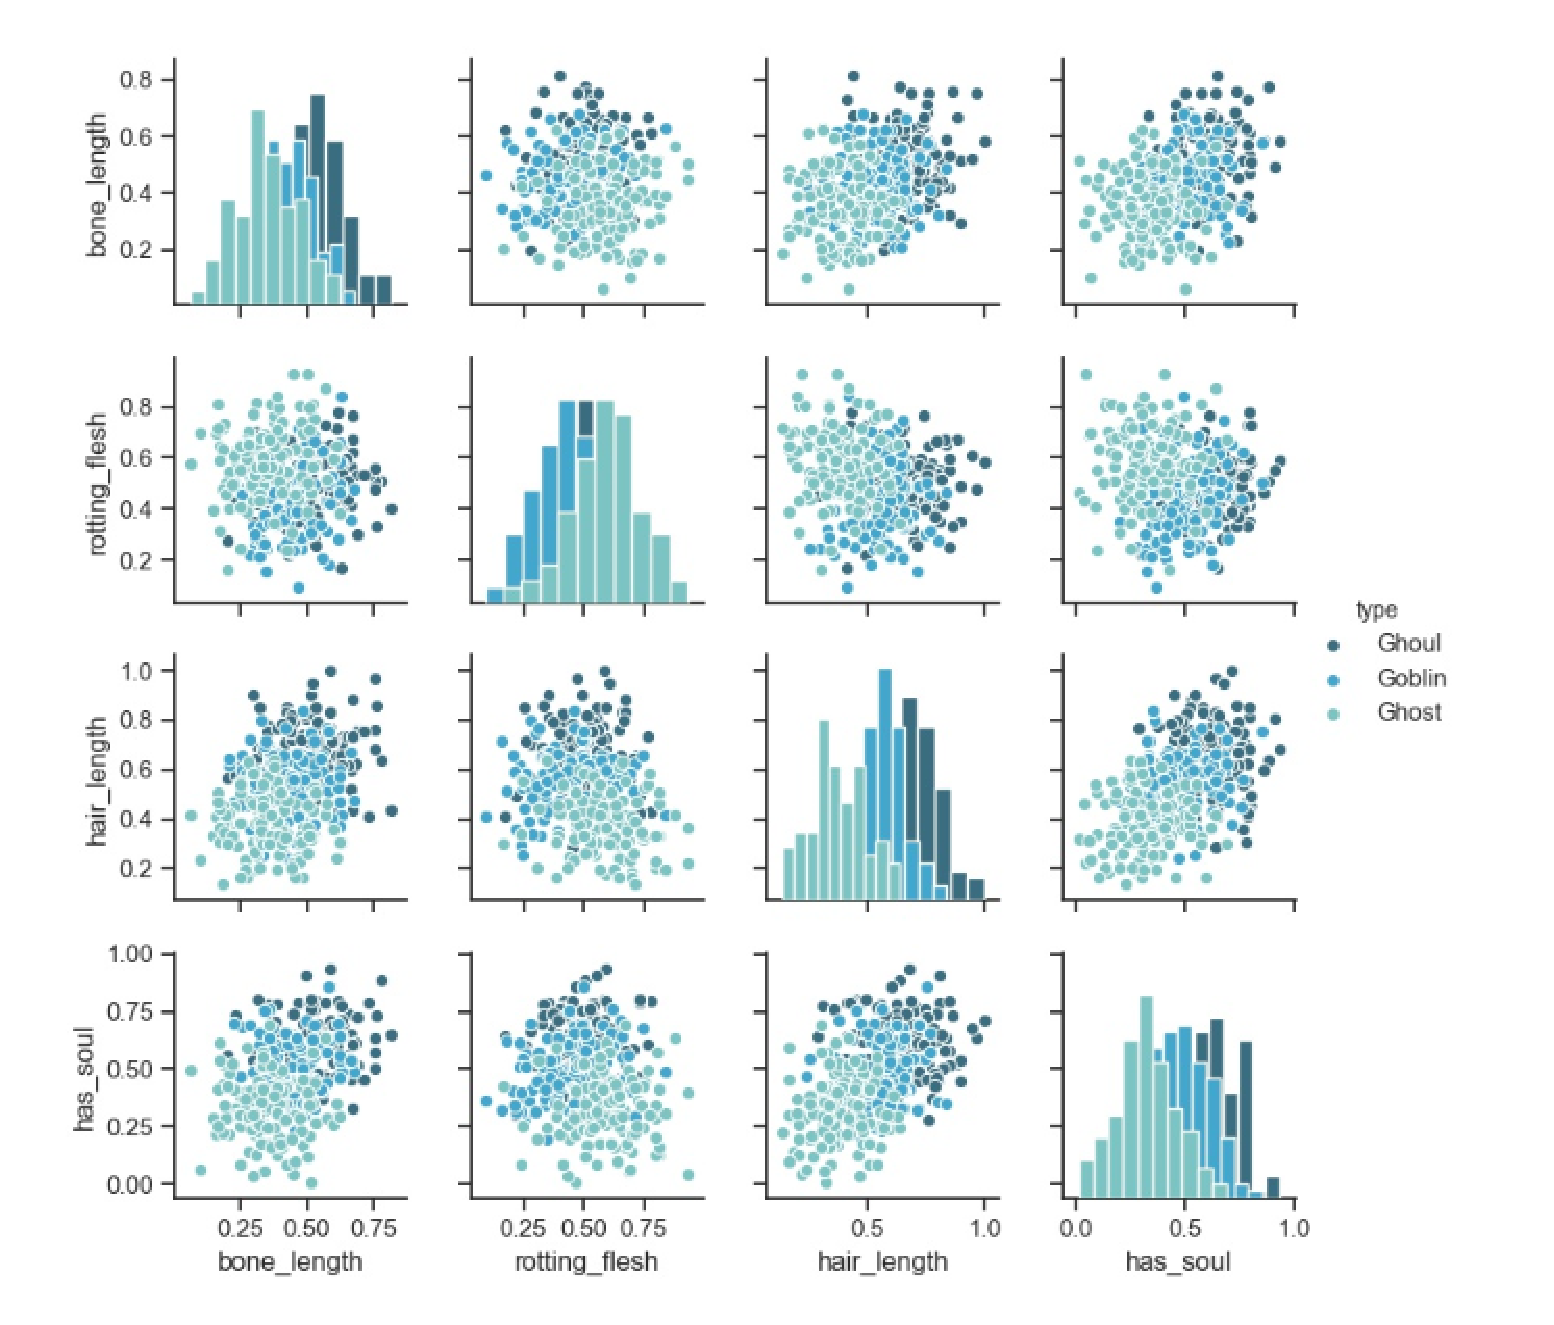
\includegraphics[scale=0.3]{5.eps}
	\caption{Feature Scatterplot}
\end{figure}


\hspace*{0.4cm}D. Correllogram\\
\hspace*{0.4cm}Correlogram is used to visually see the correlation metric between all possible pairs of numeric variables in a given dataframe. This image help us to analyze features and their impact on the 'type' column. As we can see the 'type' column has a high value of negative correlation with columns 'has_soul' and 'rotting_flesh'. Although the correlation with the 'hair_length' is not very big.\\
\begin{figure}[h]\centering
	%\graphicspath{{figures/}{mine/}}
	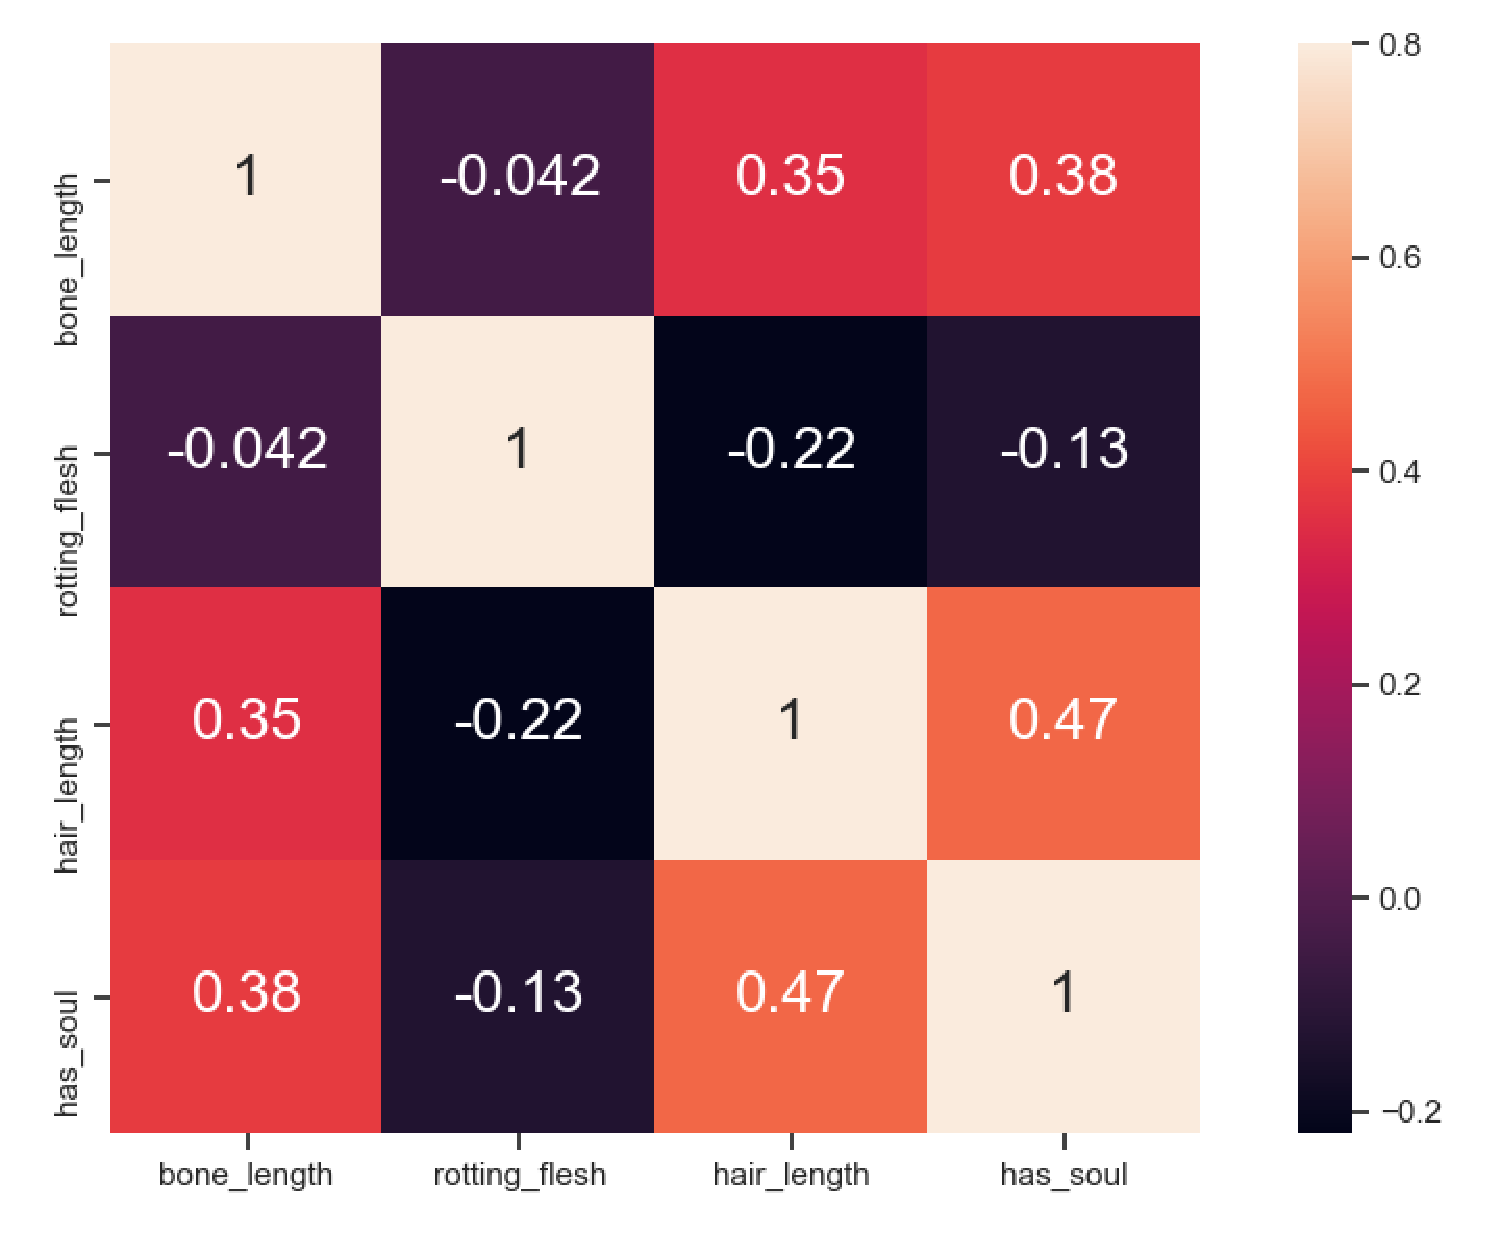
\includegraphics[scale=0.3]{7.eps}
	\caption{Correllogram}
\end{figure}

%Analyzing the correlation between other features it's possible to see that 'has_soul' and 'hair_length' have an interesting value as well as the column 'has_soul' with 'rotting_flesh'. Lets then try to extract some new features from here. 
%Test citation~\cite{BL12J01}. 
%\begin{JournalOnly}
%and~\citep{BJL11J01} or~\citet{BJL11J01}.
%\end{JournalOnly}

%This is for~\cref{tbl:overall-experiments}, 
%\todo[fancyline]{Testing.}
%and this is for~\cref{sec-conclusions}.
%\todo[noline]{A note with no line back to the text.}%
%\gangli{This is comment from Gang.}
%\qwu{Response from QW}

Number:
\num{123}.
\numlist{10;30;50;70},
\numrange{10}{30},
\SIlist{10;30;45}{\metre},
and
\SI{10}{\percent}

\missingfigure[figcolor=white]{Testing figcolor}


\begin{ConferenceOnly}
We have \SI{10}{\hertz},
\si{\kilogram\metre\per\second},
the range: \SIrange{10}{100}{\hertz}.
$\nicefrac[]{1}{2}$.

\missingfigure{Make a sketch of the structure of a trebuchet.}

\end{ConferenceOnly}


For~\cref{eq:test},
as shown below:

\begin{equation}\label{eq:test}
a = b \times \sqrt{ab}
\end{equation}

\blindmathpaper

\section{Preliminaries} \label{sec-preliminaries}

\blindtext

\gliMarker  %TODO: GLi Here


\section{Method} \label{sec-method}

\blindtext
\blindlist{itemize}[3]
\blinditemize
\blindenumerate

\blindmathtrue
\blindmathfalse
\blinddescription

\qwuMarker %TODO: QWu Here

\section{Experiment and Analysis} \label{sec-experiment}


\begin{table}  \centering
  \caption{Precision Comparison on Event Detection Methods}
  \label{tbl:overall-experiments}
  \begin{tabular}{cccc}
\toprule
    % after \\: \hline or \cline{col1-col2} \cline{col3-col4} ...
    & OR Event Detection & AC Event Detection & TC Event Detection \\
\midrule
    precision & 0.83 & 0.69 & 0.46 \\
    recall & 0.68 & 0.48 & 0.36 \\
    F-score & 0.747 & 0.57 & 0.4 \\
\bottomrule
\end{tabular}
\end{table}


\section{Conclusions} \label{sec-conclusions}

\blindtext

\section*{Acknowledgment}

\lipsum[1]


The authors would like to thank \ldots

